\documentclass[11pt]{article}

\usepackage[margin=1.05in]{geometry}
\usepackage{amsmath,amssymb}
\usepackage{booktabs}
\usepackage{graphicx}
\usepackage{microtype}
\usepackage{xcolor}
\usepackage[numbers,sort&compress]{natbib}
\usepackage{caption}
\captionsetup{font=small,labelfont=bf,skip=6pt}
\usepackage[colorlinks=true,linkcolor=teal!60!black,citecolor=teal!60!black,urlcolor=teal!60!black]{hyperref}

\definecolor{brandteal}{HTML}{0E8D7C}
\definecolor{inknavy}{HTML}{1B2838}

\newcommand{\phat}{\hat{p}}
\newcommand{\version}{reference-hazard-2026.07}

\title{\textbf{An Interpretable, Calibrated, and Auditable
Behavioural Risk Model for Online Gambling Harm Detection}\\[4pt]
\large with privacy-preserving operator deployment and in-browser recalibration}
\author{Kahlil Simeon-Rose\\
\small Carson College of Business, Washington State University, Everett, WA, USA\\
\small Technical white paper, v1.0 \quad\textbullet\quad open reference implementation}
\date{July 2026}

\begin{document}
\maketitle

\begin{abstract}
\noindent
We describe the risk model and system architecture of an
open, white-label responsible-gambling (RG) analytics platform that scores online
gambling accounts for behavioural risk. The model is interpretable by construction: a
player's 0--100 risk index is a non-negative weighted mean of thirteen
literature-anchored behavioural markers, and a separate discrete-time hazard layer
maps that index to a calibrated probability of the harm proxy within twelve months. Marker weights are fitted on a large
longitudinal research cohort of online bettors (subsequent RG-coded account closure as
the outcome) under a leakage-aware prospective design, blending a monotonic
(non-negative) multivariate logistic fit with per-marker univariate discrimination so
that redundancy is down-weighted without eliminating any clinically grounded marker.
The deployed rule attains ROC-AUC $0.673$ against ever-exclusion and $0.711$ at the
twelve-month horizon (multivariate ceiling $0.688$; PR-AUC $0.109$ against a $0.048$
base rate), with well-calibrated twelve-month probabilities (Brier $0.023$, ECE $0.003$).
A distinct human-in-the-loop overlay folds structured staff observations into the score
with incremental-information weighting, a bounded corroboration uplift, and a standing
disclosure floor that clears only on human follow-up. The platform is designed for
operator self-deployment: data onboarding with automatic column mapping, entirely
client-side re-fitting and recalibration on operator-labelled outcomes (no data
egress), a tamper-evident hash-chained audit trail, model cards with composition
versioning, and fairness audits that include the discretionary observation channel.
All components ship as an open reference implementation on synthetic data.
\end{abstract}

\section{Introduction}\label{sec:intro}

Gambling operators are increasingly required---by regulation, licensing condition, or
their own safer-gambling commitments---to identify accounts at elevated risk of
gambling-related harm early enough to intervene. Vendor solutions in this space are
typically proprietary: model structure, training labels, validation results, and
failure modes are not inspectable by the operator, the regulator, or the research
community. This sits uncomfortably with two facts. First, high-stakes decisions about
individual people are involved, which argues for models that are interpretable rather
than post-hoc explained \citep{rudin2019}. Second, the underlying science---behavioural
markers of harm in account data---originates in the \emph{open} literature
\citep{labrie2007,braverman2012,braverman2013,haeusler2016}, so there is no fundamental
reason the operational layer must be opaque.

This work is an attempt to build the operational layer in the open. This paper
documents its risk model and the design decisions that make the system deployable by an
RG team rather than a machine-learning team. Our contributions:

\begin{enumerate}\itemsep2pt
  \item \textbf{An interpretable, calibrated two-layer score} (\S\ref{sec:model}): an
  ordinal 0--100 index (a non-negative weighted mean of thirteen behavioural markers)
  that drives five monitoring tiers, plus a separately reported calibrated probability
  of the harm proxy. Keeping the layers distinct avoids the tier collapse that occurs
  when rare-outcome probabilities are used directly as scores.
  \item \textbf{A defensible weight-fitting recipe for collinear marker sets}
  (\S\ref{sec:fitting}): blending a monotonicity-constrained multivariate fit with
  univariate discrimination, so weights are redundancy-aware yet no canonical marker is
  zeroed by collinearity---preserving face validity for regulators and practitioners.
  \item \textbf{A human-in-the-loop overlay} (\S\ref{sec:overlay}) that treats the
  staff interaction log as a model input: observed markers corroborate the data-derived
  score under \emph{incremental-information} weighting (confirming what the data
  already shows adds little; data-blind emotional/social signal counts fully), and
  critical disclosures impose a standing floor cleared only by human follow-up.
  \item \textbf{Governance as a first-class subsystem} (\S\ref{sec:governance}):
  a tamper-evident hash-chained audit of every score-affecting action, model cards with
  composition versioning \citep{mitchell2019}, a global toggle between the validated
  data-only score and the combined score, and fairness audits that cover the
  discretionary observation channel.
  \item \textbf{Privacy-preserving operator deployment} (\S\ref{sec:deployment}):
  column-mapped data onboarding and full model re-fitting/recalibration executed in the
  operator's browser, so account-level data never leaves their environment.
\end{enumerate}

\begin{figure}[t]
  \centering
  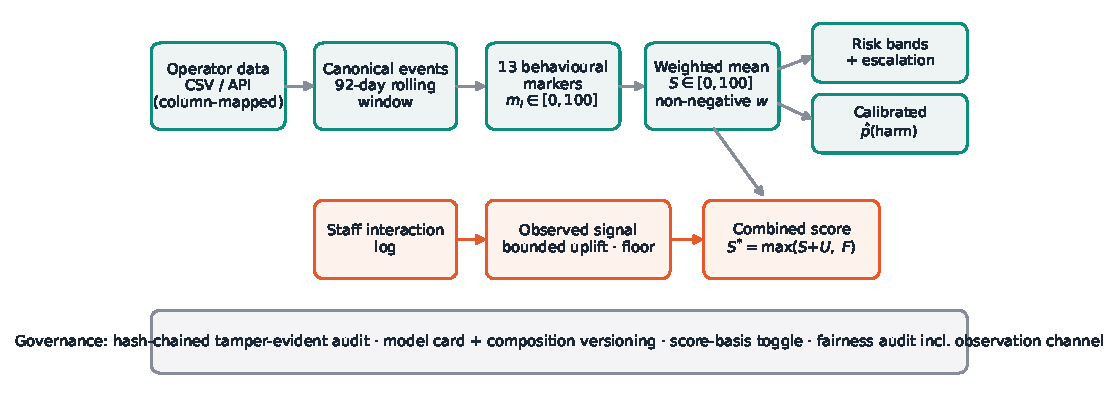
\includegraphics[width=\textwidth]{figures/fig_pipeline.pdf}
  \caption{System architecture. The data lane (top) computes thirteen behavioural
  markers over a rolling 92-day window and aggregates them into the ordinal index $S$,
  which maps to monitoring tiers and, through a separate calibration layer, to
  $\phat(\text{harm})$. The human lane (middle) folds structured staff observations
  into a combined score via a bounded uplift and a disclosure floor. All
  score-affecting actions feed the governance layer (bottom).}
  \label{fig:pipeline}
\end{figure}

\section{Background}\label{sec:background}

\paragraph{Behavioural markers.} Longitudinal studies of online-gambling account
data established that early betting behaviour separates players who later exhibit
harm-adjacent outcomes: Braverman and Shaffer \citep{braverman2012} identified
frequency, intensity, variability, and trajectory markers in the first month of play;
later work added cross-game involvement (``breadth'') as an independent signal
\citep{braverman2013,laplante2014}. Payment behaviour is similarly informative:
Haeusler \citep{haeusler2016} showed deposit and withdrawal patterns (including reversed
withdrawals and the number of payment methods) predict future self-exclusion, and
account holders flagged by corporate RG programmes show distinctive transaction
patterns \citep{gray2012}. Machine-learning replications reach comparable conclusions
with deposit-frequency features among the strongest predictors
\citep{percy2016,finkenwirth2021,ukhov2021,hopfgartner2023}.

\paragraph{Labels.} There is no direct ground-truth label for gambling harm in account
data. The pragmatic proxy is voluntary self-exclusion or RG-coded account closure, but
it is \emph{under-ascertained}: many harmed players never self-exclude, and motivations
for closure vary \citep{catania2021}. Formally this is a positive--unlabeled (PU)
learning problem \citep{elkan2008}: observed positives are reliable, but negatives are
a mixture. This shapes evaluation (rank metrics over accuracy; recall-oriented
operating points; false positives are expected rather than errors) and communication
(the model detects \emph{similarity to players who later self-excluded}, not harm
itself).

\paragraph{Interpretability and calibration.} For consequential decisions,
Rudin \citep{rudin2019} argues for models interpretable by construction rather than
post-hoc explanation of black boxes. Independently, scores used for resource allocation should
be \emph{calibrated}---predicted probabilities should match observed frequencies
\citep{platt1999,niculescu2005,guo2017}. Both properties are design requirements here.

\section{Data and label construction}\label{sec:data}

We fit default weights on a large longitudinal account-level cohort of online bettors
assembled for research use; the fitting extract is not redistributed with the
product.\footnote{The shipped product contains no cohort records: its demonstration
portfolio is synthetic, generated from aggregate distributions only
(\S\ref{sec:reference}).} It combines daily betting aggregates, deposit and withdrawal
transactions, and RG-event records, structurally comparable to the account data used
throughout the behavioural-markers literature \citep{labrie2007,braverman2012}.

\paragraph{Prospective windows.} Each account is anchored at its first observed
activity; features are computed over the following 90 days. The label is an RG-coded
account closure (typically customer-initiated self-exclusion)
occurring \emph{strictly after} the feature window, with event timing retained for
the hazard layer (\S\ref{sec:calibration}). Accounts whose closure falls inside
the window are dropped as ambiguous rather than labelled, eliminating outcome leakage
into features. The runtime product mirrors this design with a 92-day rolling window.

\paragraph{Modelling set.} Roughly ten thousand accounts, with outcome prevalence of
approximately $4.8\%$. Demographic attributes (age, sex) are \emph{deliberately excluded} from the
deployed scorer (\S\ref{sec:fairness}); an exploratory model including them is reported
only as a reference point.

\section{Behavioural markers}\label{sec:markers}

The engine computes thirteen markers, each a deterministic transform of the account's
window mapped to a bounded $[0,100]$ sub-score with a human-readable explanation
(e.g.\ ``returned to play after 31 of 33 significant loss days''). Table~\ref{tab:markers}
lists each marker, the cohort feature used as its fitting proxy, its standalone
discrimination of the label, and its fitted weight. Ten markers have direct analogs in
the cohort; three (session duration, late-night play, in-session loss-of-control) have
no analog in betting-and-payments data and enter as \emph{informed priors}, grounded in
practitioner codes and problem-gambling screens (e.g.\ PGSI loss-of-control items
\citep{ferris2001}) and assigned the median fitted weight. They are labelled as priors
in the product's model card.

\begin{table}[t]
\centering\small
\caption{Markers, fitting proxies, univariate discrimination of later RG closure
(oriented AUC and Gini), and deployed weights ($w_i$, normalised to mean ${\approx}1$
over fitted markers). Priors have no cohort analog.}
\label{tab:markers}
\begin{tabular}{@{}llcccl@{}}
\toprule
Marker & Cohort proxy & AUC & Gini & $w_i$ & Evidence \\
\midrule
Increasing loss tolerance & mean daily stake & 0.644 & 0.288 & 2.775 & \citep{braverman2012} \\
Impulsive transactions & deposits per active day & 0.627 & 0.255 & 2.232 & \citep{haeusler2016,percy2016} \\
Deposit-frequency escalation & deposit count & 0.632 & 0.263 & 1.642 & \citep{haeusler2016,finkenwirth2021} \\
Repeated loss of winnings & reversed-withdrawal amount & 0.558 & 0.116 & 1.065 & \citep{haeusler2016,gray2012} \\
Chasing losses & net loss over window & 0.589 & 0.178 & 0.813 & \citep{braverman2012,gray2012} \\
Longer session durations & --- (prior) & --- & --- & 0.636 & \citep{ferris2001} \\
Late-night play & --- (prior) & --- & --- & 0.636 & \citep{ferris2001} \\
Inability to stop & --- (prior) & --- & --- & 0.636 & \citep{ferris2001} \\
Payment-method switching & distinct payment methods & 0.550 & 0.101 & 0.459 & \citep{haeusler2016,hopfgartner2023} \\
Deposit volatility & CV of daily stake & 0.532 & 0.064 & 0.292 & \citep{braverman2012} \\
Play frequency & active days & 0.528 & 0.056 & 0.255 & \citep{labrie2007,braverman2012} \\
Shift to faster games & products played & 0.515 & 0.029 & 0.250 & \citep{braverman2013,laplante2014} \\
Increasing bet sizes & stake-trajectory slope & 0.509 & 0.018 & 0.215 & \citep{braverman2012} \\
\bottomrule
\end{tabular}
\end{table}

\section{The risk model}\label{sec:model}

\subsection{Aggregation}
Let $m_i \in [0,100]$ be the marker sub-scores and $w_i \ge 0$ their weights. The
ordinal risk index is the weighted mean
\begin{equation}
  S \;=\; \frac{\sum_i w_i\, m_i}{\sum_i w_i} \;\in\; [0,100].
  \label{eq:agg}
\end{equation}
Monotonicity is structural: no marker can lower risk, and each marker's contribution
$w_i m_i$ is directly displayable, which is what the product's explanation panels show.
An earlier hand-set aggregation (a $0.62/0.38$ blend of the weighted mean with the mean
of the top-3 markers) was removed when weights were fitted: severity concentration is
now expressed through the fitted weights themselves rather than a second heuristic.

\subsection{Weight fitting}\label{sec:fitting}
Fitting proxies are $\log(1{+}x)$-transformed, standardised, and oriented so that
larger values indicate risk. A multivariate logistic regression is fitted under a
non-negativity constraint with an $\ell_2$ penalty:
\begin{equation}
  (b, \mathbf{w}_{\mathrm{mv}}) \;=\;
  \arg\min_{b,\ \mathbf{w}\ge 0}\;
  \tfrac{1}{n}\textstyle\sum_j \ell\!\big(y_j,\ \sigma(b + \mathbf{x}_j^\top\mathbf{w})\big)
  \;+\; \lambda \lVert \mathbf{w} \rVert_2^2 .
  \label{eq:nnlogit}
\end{equation}
Constrained multivariate fitting is redundancy-aware but, under collinearity, drives
some canonical markers to exactly zero (in this cohort: chasing losses, play frequency,
deposit volatility, payment switching). A scorer that assigns \emph{zero} weight to
chasing losses would be statistically defensible yet unacceptable on face validity to
practitioners and regulators, and brittle if a zeroed marker's correlated proxy is
missing in an operator's data. We therefore blend with per-marker univariate
discrimination $g_i = 2\max(\mathrm{AUC}_i,\,1{-}\mathrm{AUC}_i) - 1$:
\begin{equation}
  \mathbf{w} \;=\; \mathcal{N}\!\Big( \tfrac{1}{2}\,\mathcal{N}(\mathbf{w}_{\mathrm{mv}})
  + \tfrac{1}{2}\,\mathcal{N}(\mathbf{g}) \Big),
  \qquad
  \mathcal{N}(\mathbf{v}) = \mathbf{v} \big/ \operatorname{mean}(\mathbf{v}_{+}),
  \label{eq:blend}
\end{equation}
yielding the weights of Table~\ref{tab:markers} (Figure~\ref{fig:weights}): every
literature-grounded marker retains non-trivial weight, while redundant markers are
substantially down-weighted relative to their univariate rank.

\begin{figure}[t]
  \centering
  \begin{minipage}[t]{0.52\textwidth}
    \centering
    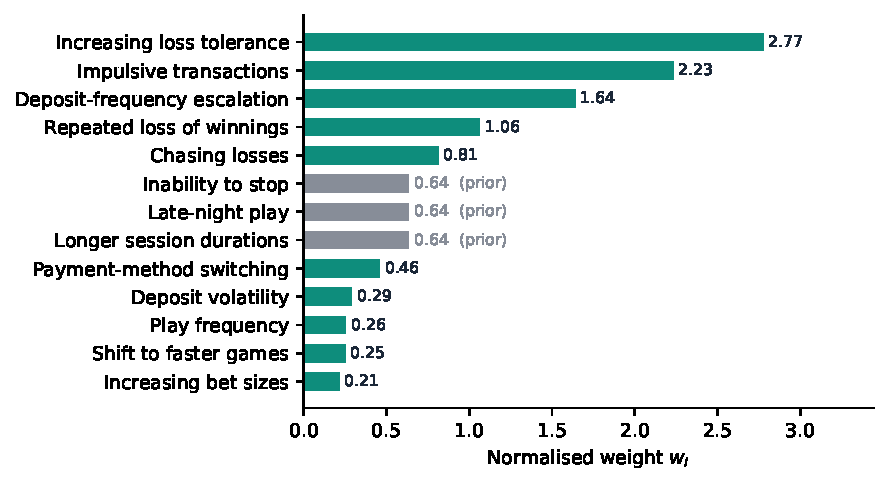
\includegraphics[width=\linewidth]{figures/fig_weights.pdf}
  \end{minipage}\hfill
  \begin{minipage}[t]{0.44\textwidth}
    \centering
    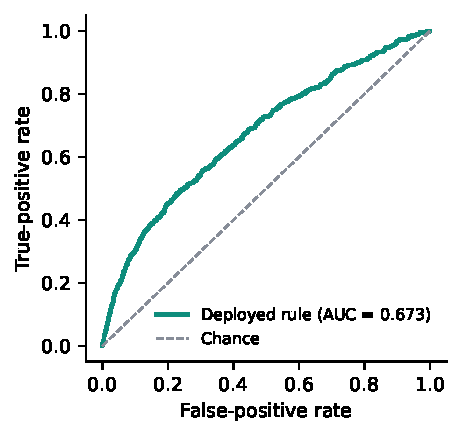
\includegraphics[width=0.72\linewidth]{figures/fig_roc.pdf}
  \end{minipage}
  \caption{\textbf{Left:} deployed marker weights (grey = literature priors with no
  cohort analog). \textbf{Right:} ROC of the deployed weighted-mean rule on the
  fitting cohort.}
  \label{fig:weights}
\end{figure}

\subsection{Calibration and score presentation}\label{sec:calibration}
The probability layer is a \emph{discrete-time hazard} on the index. With months
$j = 1, 2, \dots$ after the feature window grouped into pieces
$\pi(j) \in \{\text{1--3}, \text{4--6}, \text{7--12}, \text{13--24}, \text{25--36}\}$,
\begin{equation}
  h(j \mid S) \;=\; \sigma\!\big(\alpha_{\pi(j)} + \beta\, S/100\big),
  \qquad
  \phat_{H} \;=\; 1 - \prod_{j=1}^{H} \big(1 - h(j \mid S)\big),
  \label{eq:calib}
\end{equation}
reported at the $H{=}12$-month horizon. Events are RG-coded closures dated after the
window; accounts are censored at the administrative end of the records or at 36
months. This replaces the earlier binary layer and fixes its two defects: short
follow-up no longer masquerades as a clean negative, and a closure three weeks after
the window is no longer the same label as one three years later. The fitted monthly
baseline ($\hat{\alpha} = -9.03,\ -8.72,\ -8.61,\ -9.77,\ -10.12$;
$\hat{\beta} = 4.50$) peaks in months 4--12 and declines thereafter; the single
slope on $S$ is a proportional-hazards-style assumption accepted for
interpretability.

Because the outcome is rare, twelve-month probabilities are small even for the
riskiest accounts ($\phat_{12} \approx 0.5\%$ at $S{=}20$, $1.2\%$ at $S{=}40$,
$2.9\%$ at $S{=}60$, $6.9\%$ at $S{=}80$). Using $100\,\phat$ as ``the score''
would compress the whole portfolio into the lowest monitoring tier. The product
therefore presents \emph{two} numbers with distinct semantics: the ordinal index $S$
(drives tiers, queues, escalation) and $\phat_{12}$ (the absolute-risk read, shown
alongside). Tier cut-points
($20/38/52/66$ for Moderate/Elevated/High/Critical) are re-anchored to the deployed
score distribution so all five tiers are populated as a monitoring pyramid; operators
and jurisdiction rule-packs may override them.

\subsection{Performance}\label{sec:performance}

\begin{table}[t]
\centering\small
\caption{Performance on the fitting cohort (prevalence ${\approx}4.8\%$). The
deployed rule's discrimination is evaluated in-sample; the unblended constrained model
is additionally evaluated out-of-fold (5-fold). Calibration metrics are 5-fold
out-of-fold at the twelve-month horizon with the hazard layer re-learnt per fold
(weights fixed).}
\label{tab:perf}
\begin{tabular}{@{}lc@{}}
\toprule
Metric & Value \\
\midrule
ROC-AUC, deployed rule (Eq.~\ref{eq:agg}--\ref{eq:blend}) & 0.673 \\
ROC-AUC, constrained multivariate (5-fold OOF / in-sample) & 0.684 / 0.688 \\
ROC-AUC, exploratory unconstrained logistic incl.\ demographics (5-fold OOF) & 0.700 \\
PR-AUC (base rate 0.048) & 0.109 \\
ROC-AUC at the 12-month horizon & 0.711 \\
Brier, hazard-calibrated $\phat_{12}$ (5-fold OOF) & 0.0226 \\
Expected calibration error, $\phat_{12}$ (10 bins over support) & 0.003 \\
Precision at recall $=0.80$ & 0.062 \\
Recall in top score decile (lift) & 0.288 ($2.9\times$) \\
\bottomrule
\end{tabular}
\end{table}

Table~\ref{tab:perf} summarises performance; Figure~\ref{fig:reliability} shows the
reliability diagram. Three observations. First, the deployed rule sits within
$0.015$ AUC of its own multivariate ceiling: the interpretable weighted mean gives up
almost nothing relative to the constrained model it is derived from, and the small
parameter count ($13$ bounded weights on ${\sim}10^4$ observations) plus the OOF/in-sample
agreement ($0.684$ vs $0.688$) indicates negligible overfitting. Second, forgoing
demographic features and sign flexibility costs ${\sim}0.027$ AUC against the
unconstrained reference---the price of monotonicity and demographic neutrality, which
we accept by design. Third, these discriminations are consistent with published
self-exclusion prediction on comparable features and horizons
\citep{percy2016,finkenwirth2021,hopfgartner2023}; under an under-ascertained label
\citep{catania2021}, measured AUC also \emph{understates} true separation, since an
unknown fraction of ``negatives'' are unlabelled positives \citep{elkan2008}.
Operationally, a team reviewing the top decile of scores reaches $28.8\%$ of all future
RG closures at $2.9\times$ base-rate precision.

\begin{figure}[t]
  \centering
  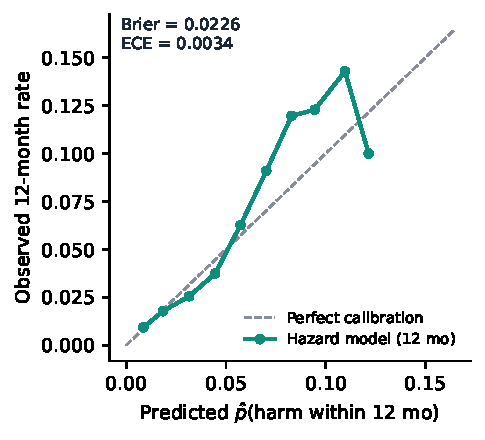
\includegraphics[width=0.4\textwidth]{figures/fig_reliability.pdf}
  \caption{Reliability of the calibrated $\phat$ (5-fold out-of-fold, calibration
  re-learnt per fold). The in-app model card reports ECE $= 0.004$ under coarser
  unit-interval binning; the support-binned value shown here is the stricter figure.}
  \label{fig:reliability}
\end{figure}

\section{The staff-observation overlay}\label{sec:overlay}

Account data cannot see distress, self-disclosed concern, or a family member's phone
call---signals that venue and support staff observe directly and that practitioner
codes treat as high-priority \citep{delfabbro2012}. The platform therefore maintains a
structured interaction log (observations, player-health conversations, interventions,
referrals, follow-ups, each tagged with observed markers from a 15-marker taxonomy in
five categories: behavioural, financial, time, emotional, social) and folds it into the
score as an explicit, bounded overlay---never silently.

\paragraph{Incremental-information weighting.} Each observed marker $o$ carries weight
$\omega_o$, a kind multiplier $\kappa \in [0.6, 1.0]$ (a referral outranks a passing
observation), recency decay $\rho(\Delta t) = 2^{-\Delta t / 30\,\mathrm{days}}$, and an
\emph{information factor}
\begin{equation}
  \iota_o \;=\;
  \begin{cases}
    1 & \text{no data analog (e.g.\ emotional/social markers)}\\[2pt]
    \max\!\big(0.15,\; 1 - d_o/100\big) & \text{data analog with sub-score } d_o,
  \end{cases}
\end{equation}
so an observation that merely confirms a marker the data already scores highly adds
almost nothing, while one contradicting a low data score (a blind spot, e.g.\ retail
cash play) or with no data analog carries full weight. This prevents observation
\emph{intensity}---how closely a venue watches---from inflating scores by itself.
The total load $L = \sum \omega_o\,\kappa\,\rho\,\iota_o$ saturates into a bounded
corroboration uplift $U = 18 \cdot \big(1 - e^{-L/1.9}\big)$, capped so the validated
data layer remains primary.

\paragraph{Standing disclosure floor.} A critical disclosure (self-disclosed concern;
third-party concern) imposes a floor $F = 50$ (the Elevated tier) on the combined
score. The floor does not decay with the calendar: it clears only when a staff
follow-up records the concern as resolved---and a ``checked, no concern'' follow-up
additionally dampens the corroboration load ($L \leftarrow 0.35 L$), making the overlay
a two-way ratchet rather than a monotone accumulator of suspicion. The combined score
is
\begin{equation}
  S^{*} \;=\; \min\!\big(100,\ \max(S + U,\ F)\big),
\end{equation}
with $S$ retained, displayed, and separately filterable throughout the product.

The overlay is deliberately \emph{not} statistically fitted---its weights are informed
priors---and every governance surface labels it as such (\S\ref{sec:governance}). Its
effects are individually auditable: each combined score decomposes on screen into
``data-derived $S$ $+$ observations $U$'' or ``disclosure floor $F$''.

\section{Operator deployment}\label{sec:deployment}

The platform is built so that an RG analyst---not a data team---can go from an
operator's raw export to a calibrated deployment.

\paragraph{Cold start.} The shipped model (\texttt{\version}) works with no operator
data at all: weights and calibration come from the reference-cohort fit above, and the
demonstration portfolio is synthetic.

\paragraph{Data onboarding.} Operators upload up to four CSVs (identities, daily
wagers, wallet transactions, sessions). Headers are matched to the canonical schema by
an alias dictionary (e.g.\ \texttt{CustomerRef} $\to$ \texttt{player\_id}), common
value spellings are coerced (\texttt{deposit} $\to$ \texttt{DEP}; \texttt{settled}
$\to$ \texttt{S}; \texttt{Male} $\to$ \texttt{M}), and the analyst
confirms the pre-filled mapping with live sample previews---no spreadsheet surgery.
Row-level validation and cross-file referential checks run before scoring. An optional
\texttt{self\_excluded} column carries outcome labels.

\paragraph{In-browser recalibration.} With labelled data present, the platform re-fits
\emph{both} layers---non-negative marker weights (projected gradient descent on
Eq.~\ref{eq:nnlogit}) and the calibration---entirely client-side,
evaluates on a deterministic 75/25 holdout (ROC-AUC, PR-AUC, Brier, ECE, reliability
curve) against the active model, and lets the operator adopt or roll back the result. Operator re-fits currently
learn a binary logistic calibration; the time-aware hazard layer
(Eq.~\ref{eq:calib}) re-fits once date-labelled outcomes are supplied.
When the labelled set is large enough ($\geq 40$ positives), the re-fit additionally
learns \emph{monotone per-marker shapes} --- quantile-binned outcome rates smoothed by
pool-adjacent-violators --- trains a shaped candidate alongside the plain one, and
adopts shapes only if they beat the plain fit on the same holdout by at least $0.005$
AUC. The guard is not decorative: on the reference cohort an additive-monotone model
attains an out-of-fold AUC of $0.679$, \emph{no better} than the plain constrained fit
($0.684$), so there shapes would correctly be rejected; they exist for operator
distributions where marker--outcome relationships are materially non-linear. Shapes
are always learned from the operator's own distribution --- shapes fitted to cohort
proxies would not transfer --- so the shipped reference model carries none.
The adopted model is a portable versioned artifact
$\{\text{weights},\ \text{calibration},\ \text{metrics},\ \text{provenance}\}$; the
whole portfolio re-scores on adoption. Because parsing, validation, scoring, and
fitting all execute in the browser, \textbf{no account-level data leaves the operator's
environment}---a deliberately conservative posture for a domain where the training
label itself is sensitive.

\paragraph{Benchmark cards.} Any deployment can export an anonymised
\emph{benchmark card} (model version, weights, shapes, calibration, holdout metrics,
cohort size and prevalence---no account-level data), enabling cross-operator
comparison of re-fits and an empirical answer to the transportability question of
\S\ref{sec:limitations} without any data sharing.

\section{Governance, auditability, and fairness}\label{sec:governance}

\paragraph{Tamper-evident audit.} Every score-affecting action (interventions,
resolutions, and staff observations) appends to a hash chain,
\begin{equation}
  h_k = \mathrm{SHA\text{-}256}\big(h_{k-1} \,\Vert\, \mathrm{canonical}(e_k)\big),
  \qquad h_0 = 0^{64},
\end{equation}
with deterministic canonical serialisation, in the spirit of cryptographic
time-stamping \citep{haber1991}. Any retroactive edit or deletion breaks every
subsequent link; the product exposes one-click replay verification and exports the
chain (with hashes) for regulatory review. The audit log thereby \emph{is} the
compliance evidence rather than a mutable table.

\paragraph{Model cards and composition versioning.} The governance surface publishes a
model card \citep{mitchell2019}: cohort, design, per-marker weights and evidence,
validation metrics, limitations, and version history. Because the shipped score is a
composition---validated data layer plus heuristic overlay---the card versions the
composition explicitly (\texttt{\version{} + observed-v1}) and states plainly which
layer is validated and which is not. A global toggle switches every surface between the
combined score and the validated data-only score.

\paragraph{Fairness.}\label{sec:fairness} The deployed scorer uses no demographic
attributes by construction; fairness is audited post hoc instead: flag-rate parity
across subgroups, equal-opportunity recall \citep{hardt2016}, and per-tier calibration
against outcomes. Distinctively, the audit also covers the \emph{observation channel}:
because staff attention is discretionary, the platform reports observation rates, mean
observed uplift, and disclosure-floor incidence by subgroup---surfacing whether human
attention, rather than behaviour, is driving score differences. To our knowledge
commercial RG tools do not audit this channel, despite staff identification of problem
gamblers being known to be noisy \citep{delfabbro2012}.

\section{Reference implementation}\label{sec:reference}

The reference implementation is a client-side web application (React\,/\,TypeScript)
structured as ports-and-adapters around a canonical event schema, so ingestion sources,
scoring engines, and audit sinks are swappable seams rather than forks. The
demonstration portfolio is fully synthetic: 250 deterministic accounts drawn from
behavioural archetypes over illustrative, generic aggregate distributions (round
values, not derived from the reference cohort or any other dataset), with
seeded staff interactions exercising both overlay paths (corroboration and
disclosure-driven detection). Under the deployed weights and cut-points the synthetic
portfolio occupies all five tiers (79\,/\,99\,/\,40\,/\,31\,/\,1 from Low to
Critical). Beyond the model surfaces, the implementation ships \emph{jurisdiction
rule-packs} (per-jurisdiction helpline, minimum age, regulator, and mandatory
statement, applied in intervention workflows and the regulator report pack; shipped as
illustrative defaults to be verified per deployment) and a \emph{structural game-risk
lens} (an instrument scoring games' structural characteristics --- event frequency,
bet structure, volatility --- crossed with player-risk exposure), so game- and
player-level risk can be read together. Determinism is enforced throughout (seeded generators; no wall-clock or
randomness in scoring paths), so identical inputs always reproduce identical scores,
tiers, and audit hashes---a property we consider part of auditability.

\section{Limitations and future work}\label{sec:limitations}

\begin{enumerate}\itemsep2pt
  \item \textbf{Label validity.} RG-coded closure is an under-ascertained,
  behaviourally narrow proxy for harm \citep{catania2021}. Weights fitted to it
  inherit its biases; the PU framing mitigates interpretation but not the label itself.
  Fitting to richer operator outcomes (complaints, affordability failures, clinical
  referrals) via the in-browser path is the intended remedy.
  \item \textbf{Marker sub-scores are heuristics.} Only the weights and calibration are
  fitted; the $[0,100]$ marker transforms themselves are rule-based. The re-fit path
  can now learn monotone per-marker shapes from operator labels (holdout-guarded,
  \S\ref{sec:deployment}), but on the reference cohort such shapes add nothing
  ($0.679$ vs.\ $0.684$ OOF AUC), so the default transforms remain the rule-based ones.
  \item \textbf{Three markers are priors.} Session-duration, time-of-day, and
  in-session loss-of-control markers have no analog in the fitting cohort and carry
  median weight by assumption. Operators whose data includes sessions can re-fit them
  out of prior status.
  \item \textbf{Offline calibration is proxy-based.} The default calibration was
  fitted on rank-based cohort proxies of the runtime markers; the mapping is exact only
  after an operator recalibrates on their own scored population, which the product
  makes a one-click step.
  \item \textbf{The overlay is unvalidated by design.} Staff-observation weights are
  informed priors; validating them requires linked observation-outcome data that, to
  our knowledge, no public dataset provides. The overlay is therefore bounded, labelled,
  and separable everywhere.
  \item \textbf{Single-cohort weights.} The default model is fitted on one operator's
  players from one era of one product mix. Cross-operator transportability is precisely
  what the re-fit path exists to test; the product exports anonymised benchmark cards
  (metrics, weights, calibration---no account data) so deployments can compare re-fits
  as community benchmarks.
\end{enumerate}

\section{Conclusion}

This reference implementation demonstrates that a responsible-gambling risk engine can be
simultaneously \emph{evidence-based} (weights fitted to a longitudinal reference cohort
under a leakage-aware design), \emph{interpretable by construction} (a monotone
weighted mean whose every contribution is displayable), \emph{calibrated} (an explicit,
separately reported probability layer), \emph{honest about its own composition}
(validated data layer vs.\ labelled heuristic overlay, with the human channel audited
for bias), and \emph{deployable without data egress}. None of these properties required
proprietary methods. We offer the system---and this document---as a reference point for
what operators and regulators can reasonably demand of behavioural risk tooling.

\begin{thebibliography}{99}\small

\bibitem{labrie2007} LaBrie, R.~A., LaPlante, D.~A., Nelson, S.~E., Schumann, A., \&
Shaffer, H.~J. (2007). Assessing the playing field: A prospective longitudinal study of
Internet sports gambling behavior. \emph{Journal of Gambling Studies, 23}(3), 347--362.

\bibitem{braverman2012} Braverman, J., \& Shaffer, H.~J. (2012). How do gamblers start
gambling: Identifying behavioural markers for high-risk internet gambling.
\emph{European Journal of Public Health, 22}(2), 273--278.

\bibitem{braverman2013} Braverman, J., LaPlante, D.~A., Nelson, S.~E., \& Shaffer,
H.~J. (2013). Using cross-game behavioral markers for early identification of high-risk
Internet gamblers. \emph{Psychology of Addictive Behaviors, 27}(3), 868--877.

\bibitem{laplante2014} LaPlante, D.~A., Nelson, S.~E., \& Gray, H.~M. (2014). Breadth
and depth involvement: Understanding Internet gambling involvement and its relationship
to gambling problems. \emph{Psychology of Addictive Behaviors, 28}(2), 396--403.

\bibitem{haeusler2016} Haeusler, J. (2016). Follow the money: Using payment behaviour
as predictor for future self-exclusion. \emph{International Gambling Studies, 16}(2),
246--262.

\bibitem{gray2012} Gray, H.~M., LaPlante, D.~A., \& Shaffer, H.~J. (2012). Behavioral
characteristics of Internet gamblers who trigger corporate responsible gambling
interventions. \emph{Psychology of Addictive Behaviors, 26}(3), 527--535.

\bibitem{percy2016} Percy, C., Fran\c{c}a, M., Dragi\v{c}evi\'{c}, S., \& d'Avila
Garcez, A. (2016). Predicting online gambling self-exclusion: An analysis of the
performance of supervised machine learning models. \emph{International Gambling
Studies, 16}(2), 193--210.

\bibitem{finkenwirth2021} Finkenwirth, S., MacDonald, K., Deng, X., Lesch, T., \&
Clark, L. (2021). Using machine learning to predict self-exclusion status in online
gamblers on the PlayNow.com platform in British Columbia. \emph{International Gambling
Studies, 21}(2), 220--237.

\bibitem{ukhov2021} Ukhov, I., Bjurgert, J., Auer, M., \& Griffiths, M.~D. (2021).
Online problem gambling: A comparison of casino players and sports bettors via
predictive modeling using behavioral tracking data. \emph{Journal of Gambling Studies,
37}(3), 877--897.

\bibitem{hopfgartner2023} Hopfgartner, N., Auer, M., Helic, D., \& Griffiths, M.~D.
(2023). Predicting self-exclusion among online gamblers: An empirical real-world study.
\emph{Journal of Gambling Studies, 39}, 447--465.

\bibitem{catania2021} Catania, M., \& Griffiths, M.~D. (2021). Understanding online
voluntary self-exclusion in gambling: An empirical study using account-based behavioral
tracking data. \emph{International Journal of Environmental Research and Public Health,
18}(4), 2000.

\bibitem{delfabbro2012} Delfabbro, P., Borgas, M., \& King, D.~L. (2012). Venue staff
knowledge of their patrons' gambling and problem gambling. \emph{Journal of Gambling
Studies, 28}(2), 155--169.

\bibitem{ferris2001} Ferris, J., \& Wynne, H. (2001). \emph{The Canadian Problem
Gambling Index: Final report}. Canadian Centre on Substance Abuse.

\bibitem{elkan2008} Elkan, C., \& Noto, K. (2008). Learning classifiers from only
positive and unlabeled data. In \emph{Proc.\ 14th ACM SIGKDD} (pp.~213--220).

\bibitem{platt1999} Platt, J.~C. (1999). Probabilistic outputs for support vector
machines and comparisons to regularized likelihood methods. In \emph{Advances in Large
Margin Classifiers} (pp.~61--74). MIT Press.

\bibitem{niculescu2005} Niculescu-Mizil, A., \& Caruana, R. (2005). Predicting good
probabilities with supervised learning. In \emph{Proc.\ 22nd ICML} (pp.~625--632).

\bibitem{guo2017} Guo, C., Pleiss, G., Sun, Y., \& Weinberger, K.~Q. (2017). On
calibration of modern neural networks. In \emph{Proc.\ 34th ICML} (pp.~1321--1330).

\bibitem{rudin2019} Rudin, C. (2019). Stop explaining black box machine learning models
for high stakes decisions and use interpretable models instead. \emph{Nature Machine
Intelligence, 1}(5), 206--215.

\bibitem{mitchell2019} Mitchell, M., Wu, S., Zaldivar, A., Barnes, P., Vasserman, L.,
Hutchinson, B., Spitzer, E., Raji, I.~D., \& Gebru, T. (2019). Model cards for model
reporting. In \emph{Proc.\ FAT*~'19} (pp.~220--229).

\bibitem{hardt2016} Hardt, M., Price, E., \& Srebro, N. (2016). Equality of opportunity
in supervised learning. In \emph{Advances in Neural Information Processing Systems 29}.

\bibitem{haber1991} Haber, S., \& Stornetta, W.~S. (1991). How to time-stamp a digital
document. \emph{Journal of Cryptology, 3}(2), 99--111.

\end{thebibliography}

\end{document}
